\cotefile{83}
\scanpage{209}
% archive sheet number: 208
\figure{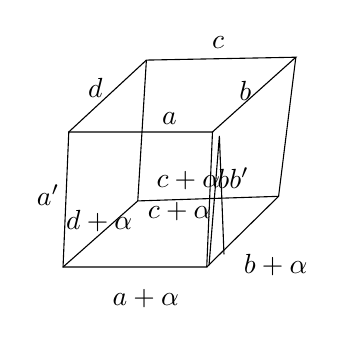
\begin{tikzpicture}[x=.73cm,y=.73cm]
\draw (0,0)--(2.5,0)--(2.6,2.35)--(.1,2.35)--cycle;
\draw (.1,2.35)--(1.45,3.6)--(4.05,3.65)--(2.6,2.35);
\draw (0,0)--(1.3,1.15)--(3.75,1.23)--(4.05,3.65);
\draw (1.3,1.15)--(1.45,3.6) (2.5,0)--(3.75,1.23);
\draw (2.54,.03)--(2.72,2.28)--(2.8,.22);
\node at (.56,3.12) {$d$}; \node at (2.7,3.9) {$c$}; \node at (3.17,3.06) {$b$};
\node at (1.85,2.58) {$a$}; \node at (-.26,1.25) {$a'$};
\node at (2.96,1.55) {$\deleted{\unsure{b}}b'$};
\node at (2.18,1.5) {$\deleted{\unsure{c+\alpha}}$}; \node at (2.03,.96) {$c+\alpha$};
\node at (.63,.80) {$\unsure{d+\alpha}$}; \node at (1.44,-.55) {$a+\alpha$};
\node at (3.7,.03) {$b+\alpha$};
\end{tikzpicture}}
\figure{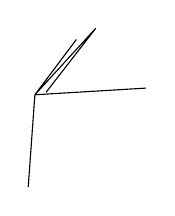
\begin{tikzpicture}[scale=.65]
\draw (0,-1.8)--(.13,0)--(2.3,.13) (.13,0)--(1.32,1.3)--(.35,.05) (.13,0)--(.94,1.08);
\end{tikzpicture}}

\figure{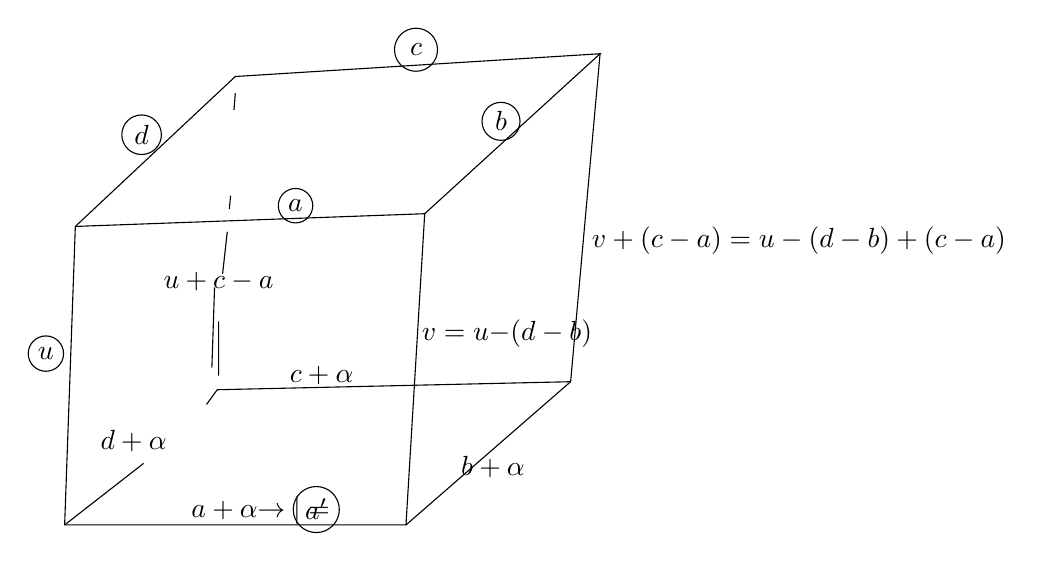
\begin{tikzpicture}[x=.85cm,y=.85cm]
\draw (0,0)--(5.1,0)--(5.38,4.65)--(.16,4.46)--cycle;
\draw (.16,4.46)--(2.55,6.7)--(8,7.04)--(5.38,4.65);
\draw (5.1,0)--(7.56,2.14)--(8,7.04);
\draw (0,0)--(1.18,.92) (2.12,1.8)--(2.28,2.02) (2.28,2.02)--(7.56,2.14);
\draw (2.2,2.35)--(2.24,3.55) (2.3,2.23)--(2.3,3.04);
\draw[thin] (2.36,3.75)--(2.43,4.38) (2.46,4.72)--(2.48,4.92) (2.53,6.20)--(2.55,6.45);
\node[draw,circle,inner sep=2pt] at (1.15,5.83) {$d$};
\node[draw,circle] at (5.25,7.1) {$c$};
\node[draw,circle,inner sep=2pt] at (6.52,6.03) {$b$};
\node[draw,circle,inner sep=2pt] at (3.45,4.77) {$a$};
\node[draw,circle,inner sep=2pt] at (-.28,2.56) {$u$};
\node at (2.30,3.64) {$u+c-a$};
\node[anchor=west] at (5.19,2.86) {$v=u\unsure{-}(d-b)$};
\node[anchor=west] at (7.73,4.25) {$v+(c-a)=u-(d-b)+(c-a)$};
\node at (1.03,1.25) {$\unsure{d+\alpha}$};
\node at (3.84,2.23) {$c+\alpha$}; \node at (6.4,.87) {$b+\alpha$};
\node at (2.93,.22) {$a+\alpha\unsure{\to|=}$};
\node[draw,circle,inner sep=2pt] at (3.76,.23) {$a'$};
\end{tikzpicture}}

\[
\begin{aligned}
&\boxed{d-b=u-v}=d-b\unsure{-}=u-v\\
&\text{i.e.}\\
&d+v=b+u\\
&d-u=b-v
\end{aligned}
\]

\[
a,b,c,d,\underset{\big|}{\alpha},u
\]
\[
\text{ou }a+\alpha=\unsure{a!|a'|a'!}
\]
\scanpage{210}
\mspage{452}
% archive sheet number: 209
années à vivre - le temps passe vit\deleted{t}e, et je vois plein de choses passionantes à faire dans ce temps qui me reste. Ça \deleted{\unsure{ne}} doit pas être bien passionant de réunir des pièces à conviction pour convaincre des juges que j'ai quelque chose à voir avec les SGA. Ce n'est pas pour eux, pas plus que pour Monsieur K.F. Springer, que je me suis fatigué à les édrire ...

Quant à ceux (à part moi-même) pour qui j'ai écrit les SGA, la relation qu'ils entretiennent à ce qui (pour moi en tous cas) reste une part de moi-même, ne m'est nullement indifférente. Elle fait partie de leur relation à ma personne. Chose étrange, je ne connais bien cette relation (ou du moins, tant soit peu) que pour mes cinq élèves cohomologistes: ceux-là même grâce auxquels il est devenu possible aujourd'hui \deleted{\unsure{qu'un Dr. K.F.}} à un Dr. K.F. Springer de m'envoyer balader, comme un \deleted{\unsure{fanfaron}}\inserted{malpropre} qui n'aurait rien à dire sur ce qu'on f\deleted{\unsure{q}}ait ou ne fait pas avec des\handwritten{\(\vert\)}textes portant le sigle SGA, que le quidam en question figure ou non sur\deleted{\unsure{t|k}} la couverture.

Le lecteur mathématicien qui m'aurait suivi jusqu'ici, et qui aurait un jour hanté les SGA (les vrais, j'entends)\deleted{\unsure{;|t}}, peut-être qu'il aura idée de me toucher un mot sur ce qu'il en pense lui-même. C'est sûr que ça me ferait plaisir de recevoir un mot de quelqu'un qui trouverait, lui, que l'ouvrage dans lequel j'ai été seul à me mettre tout entier, pendant dix ans de ma vie, et que \mbox{p\,e\,r\,s\,o\,n\,n\,e} au monde n'a eu à coeur de continuer une fois l'ouvrier parti - que cet ouvrage porte bel et bien l'empreinte de celui qui l'a conçu et porté en lui le temps qu'il a fallà, avant qu'il ne prenne forme sous ses mains et ne devienne une \mbox{m\,a\,i\,s\,o\,n} \mbox{p\,o\,u\,r} \mbox{t\,o\,u\,s}(\textsuperscript{\unsure{x|*}}). Et qu'une maison pour tous n'est pas une vespasienne dans un bas quartier, où chacun se sentirait libre de se soulager à sa guise et de griffonner ses obscénités sur des murs délabrés et poisseux ...

Et si celui qui me lit est un de ceux qui furent mes élèges, ou \deleted{qui} de ceux qui furent mes amis, et qu'il ne se sent incité à m'écrire ou à me parler, à ce sujet-là tout au moins à défaut de tout autre, qu'il sache que son silence aussi est éloquent, et qu'il sera entendu.
\scanpage{211}
% archive sheet number: 210
\[
a,b,c,d,a'\deleted{\unsure{=a+\alpha}};u
\]
\[
\alpha=a'-a
\]
\margin{\unsure{Sommation|Sommations|leurs valeurs} sur les arêtes \unsure{de chacune|de leurs|des} six faces}

\[
\begin{aligned}
S_1&=a+b+c+d\\
S'_1&=a+b+c+d+4(a'-a)=-3a+b+c\inserted{+d}+4a'\\
S_2&=\underline a+\underline u+\underline{a'}+\underline u+(\underline d-\underline b)=a-b+\cdot+d+a'+2u\\
S'_2&=\underline c+\underline u+\underline c-\underline a+\underline c+\deleted{\unsure{\alpha}}\inserted{\underline{a'}-\underline a}+\underline u-\underline d+\underline b+\underline c-\underline a\\
&=-3a+b+\deleted{\unsure{3}}4c-d+a'+2u\\
S_3&=\underline u+\underline d+\underline{a'}-\underline a+\underline u+\underline c-\underline a+\underline d=-2a+\cdot+c+2d+a'+2u\\
S'_3&=\underline b+\underline u-\underline d+\underline b+\underline b+\underline{a'}-\underline a+\underline u-\underline d+\underline b+\underline c-\underline a=-2a+4b+c-2d+a'+2u
\end{aligned}
\]

\[
\begin{array}{c}
\begin{array}{rrrrrr}a&b&c&d&a'&u\end{array}\\
\begin{pmatrix}1&1&1&1&0&0\\-3&1&1&1&4&0\\1&-1&0&1&1&2\\-3&1&4&-1&1&2\\-2&0&1&2&1&2\\-2&4&1&-2&1&2\end{pmatrix}
\end{array}
\]

\[
\begin{aligned}
\Delta={}&\det\left(\begin{smallmatrix}1&1&1&4&0\\-1&0&1&1&2\\1&4&-1&1&2\\0&1&2&1&2\\4&1&-2&1&2\end{smallmatrix}\right)
-\det\left(\begin{smallmatrix}-3&1&1&4&0\\1&0&1&1&2\\-3&4&-1&1&2\\-2&1&2&1&2\\-2&1&-2&1&2\end{smallmatrix}\right)
+\det\left(\begin{smallmatrix}-3&1&1&4&0\\1&-1&1&1&2\\-3&1&-1&1&2\\-2&0&2&1&2\\-2&4&-2&1&2\end{smallmatrix}\right)\\
&-\det\left(\begin{smallmatrix}-3&1&1&4&0\\1&-1&0&1&2\\-3&1&4&1&2\\-2&0&1&1&2\\-2&4&1&1&2\end{smallmatrix}\right)
\end{aligned}
\]
\scanpage{212}
\mspage{L 22}
% archive sheet number: 211
et sans apparence, marque un premier tournant crucial dans le témoignage, et un changement qualitatif immédiat (\textsuperscript{\unsure{x|*}}). C'était là une première chose essentielle que j'avais à apprendre, sur mon passé de mathématicien et sur moi-même. Cette connaissance d'une \mbox{p\,a\,r\,t} \mbox{d\,e} \mbox{r\,e\,s\,p\,o\,n\,s\,a\,b\deleted{\unsure{x|i}}i\,l\,i\,t\,é} qui m'incombait dans la dégradation générale (connaissance plus ou moins aigüe suivant les moments de la réflexion) est restée comme une note de fond et comme un rappel, tout au cours de Récoltes et Semaill\inserted{\handwritten{es.}} Il en a été ainsi, surtout, aux moments où ma réflexion prenait les allures d'une enquêt\deleted{\unsure{x}}e sur les disgrâpces et sur les iniquités d'une époque. Conjointement au désir de comprendre, à la curiosité donc qui anime et porte en avant tout vrai travail de découverte, c'est\unsure{x|\,\deleted{,}} cette humble connaissance (maintes fois oubliée en chemin et refaisant surface malgré tout, \deleted{\unsure{à}}\unsure{là} où on s'y attendait le moins ...) qui a préservé mon témoignage de jamais virer (je crois) à la récrimination stéri\deleted{\unsure{le}}le sur l'ingratitude du monde, voire au \char34{}\deleted{\unsure{g}}règlement de comptes\char34{} avec certains de ceux qui avaient été mes élèves ou des amis (ou les deux)\unsure{,|.}

Cette absence de complaisance vis-à-vis de moi-même m'a donné également ce calme intérieur, ou cette fortitude, qui m'ont préservé des pièges de la complaisance\inserted{ vis-à-vis d'autrui}\handwritten{,} \deleted{\unsure{(}}ou ne seraient-ce que ceux d'une fausse \char34{}discrétion\char34{}\deleted{\unsure{)}}. Tout ce que je croyais avoir à dire, à un moment ou à un autre de la réflexion, que ce soit sur moi, ou sur tel de \inserted{\handwritten{mes}} collègues, ex-élèves ou amis, ou\unsure{\_}sur un milieu, ou sur une époque, je l'ai dit, sans avoir jamais à bousculer mes réticences. Pour celles-\deleted{\unsure{c}}ci, il a suffi à chaque fois que je les examine avec attention, pour qu'elles s'évanouissent sans laisser de traces.
\scanpage{213}
% archive sheet number: 212
\figure{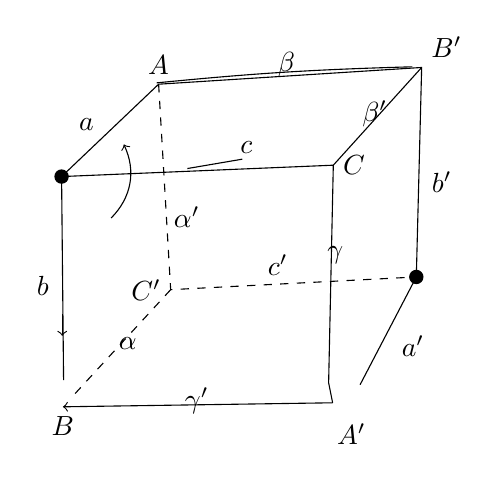
\begin{tikzpicture}[x=.85cm,y=.85cm]
\coordinate (p) at (0,3.4); \coordinate (q) at (5.3,1.9);
\fill (p) circle (2.6pt) (q) circle (2.6pt);
\draw (p)--(1.45,4.78) node[above] {$A$}--(5.38,5.03) node[above right] {$B'$}--(q);
\draw (p)--(4.06,3.57) node[right] {$C$}--(5.38,5.03);
\draw (p)--(.03,.36) (4.06,3.57)--(3.99,.32) (3.99,.32)--(4.05,.02);
\draw[->] (4.05,.02)--(.02,-.04) node[below] {$B$};
\draw (q)--(4.46,.29); \node at (4.33,-.45) {$A'$};
\draw[dashed] (1.45,4.78)--(1.63,1.71) node[left] {$C'$}--(q);
\draw[dashed] (1.63,1.71)--(.14,.09);
\draw[->] (.74,2.78) to[bend right=35] (.93,3.88);
\draw[->] (.01,1.34)--(.01,1.02);
\draw (1.42,4.8) to[bend left=2] (5.24,5.04) (1.88,3.52)--(2.7,3.66);
\node at (.37,4.18) {$a$}; \node at (3.36,5.08) {$\beta$};
\node at (4.68,4.34) {$\beta'$}; \node at (2.76,3.83) {$c$};
\node at (5.68,3.32) {$b'$}; \node at (-.28,1.77) {$b$}; \node at (1.87,2.79) {$\alpha'$};
\node at (.99,.91) {$\alpha$}; \node at (3.23,2.08) {$c'$}; \node at (4.09,2.22) {$\gamma$};
\node at (5.25,.86) {$a'$}; \node at (2.02,.05) {$\gamma'$};
\end{tikzpicture}}

\[
\gamma'-c=a'-\beta'=c'-\beta=\alpha-a\,\Big|=\delta'
\]
\[
\left\{\begin{aligned}
\gamma'&=\delta'+c\\
\beta'&=-\delta'+a'\\
\beta&=-\delta'+c'\\
\alpha&=\delta'+a
\end{aligned}\right.
\]
\margin{\unsure{restent pour compte|reste pour compte|sont pas apparus} $\underline\gamma,\underline{\alpha'}$}

\[
\underline{b-\gamma}=\underline{\alpha-a'}=\underline{\alpha'-b'}=a-\beta'\,\Big|=-\delta''
\]
\[
\begin{aligned}
\vdots\quad&\left\{\begin{aligned}
\gamma&=\deleted{\unsure{b}}+\delta''+b\\
\alpha'&=-\delta''+b'
\end{aligned}\right.\\
&\alpha=-\delta''+a'\\
&\beta'=+\delta''+a
\end{aligned}
\]
\[
\begin{aligned}
&\boxed{-\delta''+\unsure{a'|\alpha'}=\delta'+a}
\quad\tikz[baseline=(e.base)]\node[draw,ellipse,inner sep=2pt](e){$\delta'+\delta''=a'-a$};\\
&\big|\underline{+\delta''+a}=-\delta'+a'
\end{aligned}
\]
\scanpage{214}
\mspage{451}
% archive sheet number: 213
résiste pas à la tentation de la reproduire ici \inserted{(traduite)} in extenso.\deleted{\handwritten{\unsure{-}}} Il m'a fallu un moment, d'ailleurs, pour saisir que c'\deleted{\unsure{e}}était bel et bien une réponse à ma belle lettre \deleted{\unsure{d'il y avait}} du mois dernier\deleted{\unsure{,}}. \inserted{\handwritten{Voici donc la réponse.}}

Heidelberg 15.3.1985\\
\deleted{\handwritten{\unsure{\char34{}}}}Cher Professeur Grothendieck,\\

Il me faut encore vous remercier pour votre lettre du 9 février. La lettre de Mme Dr. Byrne du 15 février aura sans doute répondu à vos questions.

Rece\deleted{g}vez e\deleted{\unsure{s}}tc\\
K.F. Springer \deleted{\handwritten{\unsure{\char34{}}}}\\

Là au moins je suis fixé ! Les gens \char34{}bien informés\char34{} (dont il a été déjà question) ont dû lui expliquer que c'était pas la peine qu'il se fatigue pour le \deleted{\unsure{m}}Monsieur un peu excité qui lui écrivait là - qu'i\deleted{\unsure{b}}l ne faisait décidément pas partie du beau monde. Et c'est vrai, en plus ...

En attendant de recevoir cette réponse édifiante de la direction de l'entreprise de \deleted{\unsure{p}}Pompes \deleted{\unsure{f}}Funèbres Springer Verlag GmbH (c'était gentil encore de m'honorer d'une réponse \deleted{personelle}\inserted{signée} du directeur en personne), j'ai eu le temps de me sonder sur mes propres intentions. Le rôle joué par l'estimable entreprise me paraît vraiment très gros, et j'ai songé à l'éventualité d'un procès à gránd spectacle, où je demanderais des dommages-intérêts astronomiques, à titre de \char34{}monsieur bien\char34{}\handwritten{/}outragé, \deleted{et} victime d'inqualifiables passe\deleted{s}-droits . Mais je me suis dit aussi \deleted{que de tels pro} qu'un procès c\deleted{\unsure{d}}omme ça, ça doit bouffer une énergie\handwritten{\(\vert\)}dingue. A supposer même que j'aie gain \deleted{\unsure{d}}de cau\deleted{\unsure{d}}se et que je touche des dommages-intérêts vertigineux (soyons optimistes\unsure{)|!})\handwritten{,} au bout de X années\deleted{\unsure{,}}\inserted{\handwritten{\unsure{certes|cuites}}} - à quoi serais-je avancé ? Je ne suis pas dans le besoin et n'ai nul besoin de plus que ce que j'ai - et une escroquerie n'est pas plus ni moins une escroquerie, parce qu'un certain procès a été gagné, ou perdu. Je ne vais pas amél\deleted{\unsure{oi}}iorer le monde, ni moi-même, ni les manières de Monsieur K.F. Springer et de certains employés de l'entreprise qu'il dirige, et en tous cas pas leur\deleted{s} façon de concevoir leur métier\handwritten{,} en mobilisant des avocats et en \deleted{\unsure{leu}}\handwritten{les} faisant mobiliser les leurs\inserted{\handwritten{(*)}}. \deleted{Par contre, dans les années qui m} Et je n'améliorerai pas non plus un certain esprit dans un certain beau monde que j'ai quitté, \deleted{un}\handwritten{l'}esprit qui rend possible le genre d'opération dont le Dr. Springer et son estimable \deleted{entre} maison se \deleted{f}\handwritten{s}ont \inserted{\handwritten{faits depuis treize ans \deleted{\unsure{déjà}}}} \deleted{\unsure{l}}\handwritten{l}es serviteurs. Il me reste (je l'espère bien) quelques
\scanpage{215}
% archive sheet number: 214
\[
b-\alpha'=\gamma'-c'=\gamma-b'=\unsure{-c|c}-\beta=-\delta
\]
\[
\begin{aligned}
\alpha'&=\delta+b\\
\gamma'&=-\delta+c'\\
\gamma&=-\delta+b'\\
\beta&=\delta+c
\end{aligned}
\]
\[
\begin{aligned}
&\boxed{\deleted{\delta+b=-\delta''+b'}}\\
&\boxed{-\delta+\deleted{\unsure{\delta}}c'=\deleted{\unsure{c}}\delta'+c}\\
&\boxed{\deleted{-\delta+b'=\delta''+b}}\\
&\boxed{\delta+c=-\delta'+c'}
\end{aligned}
\]
\[
\tikz[baseline=(v.base)]\node[draw,ellipse,inner sep=2pt](v){$\begin{aligned}
\delta+\delta''&=b^{\unsure{2|\prime|+}}-b\\
\delta+\delta'&=c'-c\deleted{\unsure{\varepsilon}}
\end{aligned}$};
\]
\[
\underline{\begin{aligned}
\delta'+\delta''&=a'-a\\
\delta''+\delta&=b'-b\\
\delta+\delta'&=c'-c
\end{aligned}}
\]
\[
\boxed{\left\{\begin{aligned}
\delta&=\frac{1}{2}(-\deleted{\unsure{\delta}}\varepsilon_1+\varepsilon_2+\varepsilon_3)\\
\delta'&=\frac{1}{2}(\varepsilon_1-\varepsilon_2+\varepsilon_3)\\
\delta''&=\frac{1}{2}(\varepsilon_1+\deleted{\unsure{c}}\varepsilon_2-\varepsilon_3)
\end{aligned}\right.}
\]
\[
\delta+\delta'+\delta''=\frac{1}{2}\bigl(a'+b'+c'-(a+b+c)\bigr)
=\frac{1}{2}\bigl(\underset{\varepsilon_1}{\underline{(a'-a)}}+\underset{\varepsilon_2}{\underline{(b'-b)}}+\underset{\varepsilon_2}{\underline{(c'-c)}}\bigr)
\]
\scanpage{216}
\mspage{450}
% archive sheet number: 215
(Ce n'est pas \inserted{\handwritten{certes}} la première fois \inserted{\handwritten{ni la dernière que je suis ``soufflé''}} dans cette brillante opération \char34{}au service de la science\char34{}\handwritten{...)} \deleted{\unsure{même|ni même} \illegible{3}} J'apprends par sa lettre (datée du 15 février 85) que conformément \deleted{\unsure{aux|au}} \char34{}à la façon habituelle d'agir quand un ouvrage contient des contributions de plusieurs auteurs\char34{} (sic), il n'y avait pas lieu de s'adresser plus spécialement à moi, qui n'étais que \uline{directeur} du Séminaire ... \deleted{\unsure{(}}Les cinq \char34{}auteurs\char34{} de SGA 5 sont Bucur, Houzel, Illusie, Jouanolou, Serre, à l'exclusion de ma modeste personne, qui \deleted{\unsure{ne}} ne figure que comme \char34{}directeur\char34{} - sans doute purement honorifique, en \inserted{\handwritten{av}}ai\inserted{\handwritten{s}}-je trop dit (\textsuperscript{\unsure{x|*}}) - pour ce brillant séminaire.

Dès avant de recevoir cette lettre instructive et trouvant le temps long (n'ayant rien reçu pendant un mois), j'ai pris ma plus belle plume (en allemand) pour écrire au Dr. K.F Springer en personne, \inserted{\handwritten{lequel}} fai\deleted{sant}\handwritten{t} partie des directeurs responsables de la maison Springer. Ça a été une belle \deleted{let} lettre de deux pages machine, lui expliquant que j'étais bien peiné d'une \unsure{L|l}ongue série de désagréments dans ma relation à la maison Springer, et au delà de celles-ci, d'un certain nombre d\deleted{\unsure{1}}irrégularités grossières à mon égard, dont je me contentais pour le moment de lui soumettre deux, qui me p\deleted{\unsure{e}}araissaient particulièrement flagrant\deleted{\unsure{s}}\handwritten{es}: la publication de deux volumes des Lecture Notes (n\textsuperscript{\uline{o}}s 288,589) parus sous mon nom et sans \deleted{\unsure{aucun}} juger nécessaire de me consulter. Que dans ces deux \deleted{cas}\inserted{textes}, les idées, méthodes et résultats que j'avais développés dans les séminaires ora\uline{u}x, étaient raccourcis ou mutilés parfois au point d'être méconnaissables. Que la coïncidence de ce dernier fait, \handwritten{avec} \deleted{d}\handwritten{l}es circonstances inhabituelles qui ont entouré la publication de ces deux volumes, ne pouvait être pour moi l'effet d'un pur hasar\deleted{\unsure{s}}d. Et que je m'attendais à des excuses publiques\deleted{\unsure{d} de la part} et sans réserve de la part de la maison\handwritten{/}Springer, sous une forme qui serait à fixer d'un commun accord, une fois \deleted{que la question}\inserted{qu'un accord} de principe \deleted{ét}\handwritten{ser}ait acquis. Que j'espérais qu'il aurait à coeur comme moi de mettre fin à une situation déplaisante et inadmissible et de trouver une solution\unsure{n}qui soit à la hauteur des circonstances (\char34{}eine dem Fall geziemende Lösung zu finden\char34{}, ce qui \deleted{est} est même plus distingué encore), \char34{}ho\deleted{\unsure{x}}chachtungsvoll\char34{} (comme il se doit) signé de ma plus belle main.

Pour jouer cartes sur table, il me semble que j'ai joué cartes sur table ! Là il ne pourra pas dire, Monsieur K.F. S\handwritten{p}ringer, \deleted{\unsure{c}}\handwritten{q}u'il \deleted{\unsure{n'a}}\handwritten{n'a} pas été informé personellement de la situation, et de première main enco\deleted{\unsure{re}}re\handwritten{,}\deleted{\unsure{é}} par nul autre que le principal intéressé lui-mê\handwritten{m}e!

Le hasard fait bien les choses: j'ai \deleted{réçu} fini par recevoir une réponse (un bon mois après\inserted{\handwritten{ encore}}) pas\unsure{,|;}plus tard que hier. C'est si court que je ne
\scanpage{217}
% archive sheet number: 216
\diagram{\begin{tikzcd}[ampersand replacement=\&,row sep=1.1em,column sep=1pt]
\alpha=\sigma_{BC'}=\frac12\bigl((a'\underline{+a})\deleted{\unsure{+}}\unsure{-}(b'-b)+(c'-c)\bigr. \& \bullet\arrow[dd,bend left=50]\\
\deleted{\unsure{\alpha}}\beta=\sigma_{AB'}=\frac12\bigl(-(a'\deleted{\unsure{+}}\unsure{-}a)+(b'-b)+\underline{(c'+c)}\bigr) \& {}\arrow[u]\\
\gamma=\sigma_{CA'}=\frac12\bigl((a'-a)+\underline{(b'+b)}-(c'-c)\bigr) \& {}\arrow[u,bend right=18]
\end{tikzcd}}
\[
\begin{aligned}
&-c'+c+2c'\\
&-b'+b\\
&-a'+a\\
&c'-c
\end{aligned}
\]
\diagram{\begin{tikzcd}[ampersand replacement=\&,row sep=1.1em,column sep=1pt]
\alpha'=\sigma_{AC'}=\frac12\bigl(-(a'-a)+\underline{(b'+b^{\deleted{\unsure{\prime}}})}+(c'-c)\bigr) \& {}\arrow[dd,bend left=50]\\
\beta'=\sigma_{CB'}=\frac12\bigl((a'+a)+(b'-b)-(c'-c)\bigr) \& \bullet\arrow[u,bend right=18]\\
\gamma'=\sigma_{BA'}=\frac12\bigl((a'-a)\deleted{\unsure{+}}\unsure{-}(b'-b)+(c'\unsure{+|-}c)\bigr) \& {}\arrow[u,bend right=18]
\end{tikzcd}}

\[
a-a'+(b'+c')
\]

\unsure{Sommation des|Sommations des|Sommes des} $\sigma_a$ sur les arêtes d'une face
\[
\left.\begin{aligned}
\varphi_a&=\deleted{\unsure{b+c+}}(a'-a)+2(b+c)\\
\varphi_b&=(b'-b)+2(a+c)\\
\varphi_c&=(c'-c)+2(a+b)
\end{aligned}\right\downarrow
\]
\diagram{\begin{tikzcd}[ampersand replacement=\&,row sep=.8em,column sep=.1em]
\varphi_{a'}^{\deleted{\unsure{\prime}}}=(b'+c')\deleted{\unsure{+}}\unsure{-}(a'-a)+b'+c'={} \& 2(b'+c')-(a'-a)\\
\varphi_{b'}=a'+c'+a'-(b'-b)+c'={} \& 2(c'+a')-(b'-b)\\
\varphi_{c'}=\unsure{(a'+b')}+a'+b'-(c'-c)={} \& 2(a'+b')-(c'-c)\\
\& \text{\deleted{\unsure{font chacun} \illegible{2} \unsure{produit}!}}\arrow[uuu,bend left=34]\arrow[uu,bend left=21]\arrow[u]
\end{tikzcd}}
\scanpage{218}
\mspage{L 21}
% archive sheet number: 217
quand ce n'était celui du dédain (\char34{}délicatement dosé\char34{}), de la dérision ou du mépris, que ce soit vis-à-vis de moi (parfois) ou (surtout) vis-à-vis de ceux qui avaient osé s'inspirer de moi (sans se douter, ce\deleted{\unsure{tt}}rtes, de ce qui les attendait) et qui ét\unsure{a}ient \char34{}classés\char34{} comme ayant partie liée à moi, par quelque décret tacite et implacable. Et à nouveau je vois apparaître ici le lien \char34{}évident\char34{} et profond, entre le \mbox{r\,e\,s\,p\,e\,c\,t} (ou l'absence de respect) pour la personne d'autrui, celui pour l'acte de création et pour certains de ses fruits \deleted{parmi} les plus délicats et les plus essentiels, et enfin le respect pour les règles les plus évidentes de l'éthique scientifique, celles qui s'enracinent dans un respect élémentaire de soi et d'autrui et que je serais tenté d'appeler les \char34{}\mbox{r\,è\,g\,l\,e\,s} \mbox{d\,e} \mbox{d\,é\,\deleted{\unsure{s}}c\,e\,n\,c\,e}\char34{} dans l'exercice de notre art. \inserted{\handwritten{Ce sont là autant d'aspects, sûrement, d'un élémentaire et essentiel ``\uline{respect} \uline{de} \uline{soi}''.}} Si j'es\deleted{\unsure{saie}}saie, en une seule formule lapidair\handwritten{e,} de faire le bilan de ce que m'a enseigné Récoltes et Semailles au sujet d'un certain monde qui fut le mien, un monde auquel je m'étais identifié pendant plus de vingt ans de ma vie, je dirais: c'est un monde qui a \mbox{p\,e\,r\,d\,u} \mbox{l\,e} \mbox{r\,e\,s\,p\,e\,c\,t} (\textsuperscript{\unsure{x|*}}).

C'était là une chose déjà fortement sentie, sinon formulée, dès les années qui avaient précédé. Elle n'a fait que se confirmer et se préciser\handwritten{,} de façon \deleted{souvent} imprévue toujours et parfois stupéfiante, tout au cours de Récoltes et Semailles. Elle est clairement apparente dès le moment\unsure{,} déjà où une réflexion de nature \char34{}philosophique\char34{} et générale devient soudain un témoignage personnel , dans la section \char34{}L'étranger bienvenu\char34{} (n\textsuperscript{\uline{o}} 9\deleted{\unsure{5|2}}, p. 18) ouvrant le chapitre déjà cité \char34{}Naissance de la crainte\char34{}\deleted{\unsure{)}}.

Cette perception n'apparaît pourtant pas sur le ton de la récrimination acerbe ou amère, mais (par la logique interne de l'écriture et par l'attitude différente que celle-ci suscite) sur celui d'une \mbox{i\,n\,t\,e\,r\,r\,o\,g\,a\,t\,i\,o\,n}: quelle a été ma propre part dans cette dégradation, dans cette perte du respect que je constate aujourd'hui ? C'est là l'interrogation principale qui traverse et porte cette première partie de\margin{\unsure{()|''}} Récoltes et Semailles, jusqu'au moment où elle se résoud finalement en une constatation claire et sans équivoque (\textsuperscript{\unsure{xx|**}}). Auparavant, \unsure{()|''}cette dégradation m\handwritten{'}était apparue comme \char34{}tombée du ciel\char34{} soudain, de façon inexplicable et d'autant plus outrageuse, intolérable. Au cours de la réflexion, je découvre qu\handwritten{'}\deleted{e} \deleted{c}e\deleted{tt}\handwritten{ll}e \deleted{dégradation} s'était \deleted{déjà} poursuivie insidieusement, sans que personne sûrement ne la décèle \deleted{\unsure{en}}autour de lui ni en lui-même, tout au \deleted{cours}\inserted{\handwritten{long}} des années cinquante et soixante, \mbox{y} \mbox{c\,o\,m\,p\,r\,i\,s} \mbox{d\,a\,n\,s} \mbox{m\,a} \mbox{p\,r\,o\,p\,r\,e} \mbox{p\,e\,r\,s\,o\,n\,n\,e}.

\deleted{Cette constat} La constatation de cet humble fait, \inserted{\handwritten{bien}} évident sûrement
\scanpage{219}
% archive sheet number: 218
\[
\begin{aligned}
&\det\left(
\begin{array}{|rrr|rrr|}
\multicolumn{1}{r}{a}&b&\multicolumn{1}{r}{c}&a'&b'&\multicolumn{1}{r}{c'}\\ \hline
-\deleted{\unsure{0}}1&2&2&1&0&0\\
2&-1&2&0&1&0\\
2&2&-1&0&0&1\\ \hline
1&0&0&-1&2&2\\
0&1&0&2&-1&2\\
0&0&1&2&2&-1\\ \hline
\end{array}\right)
=\det\begin{pmatrix}27&1\\1&27\end{pmatrix}=27^2-1\in\mathbb{Q}^{*}\\
&\hspace{13em}=(3^3)^2-1=3^6-1\\
&\hspace{13em}=728\\
&\hspace{13em}=8.91\\
&\hspace{13em}\boxed{=\deleted{\unsure{8}}2^3.7.13}
\end{aligned}
\]
\margin{\uline{premier \unsure{:|à} 3}}
\[
-1+8+8-(-4-4-4)=16+12-1=27
\]
\margin{\unsure{OK|OV|Ok}}
\[
\deleted{\unsure{-1-}}\qquad
\begin{array}{rrr}
&2&7\\&2&7\\\hline
1&8&9\\5&4&\\\hline
7&2&9
\end{array}
\]
\scanpage{220}
\mspage{L 20}
% archive sheet number: 219
\deleted{par des \unsure{épithètes}} comme \char34{}vaseux\char34{}, \char34{}mou\char34{}, \char34{}inconsistant\char34{} - ou au bout opposé \inserted{\handwritten{comme}} \char34{}trivialités\char34{}, \char34{}enfantillage\char34{}, \char34{}bombinage\char34{} ...), mais où sera extirpé également ce travail même et ses fruits: celui où sont conçues, s'élaborent et naissent les notions et les visions nouvelles. Ce sera l'époque aussi où l'exercice de notre art sera réduit à d'arides et vaines voltiges de \char34{}poids et haltères\char34{} cérébraux, aux surenchères des prouesses pour \char34{}craquer\char34{} les problèmes au concours (\char34{}de difficulté proverbiale\char34{}) - l'époque d'une hypertrophie \handwritten{``}supermacho\handwritten{''} fiévreuse et stérile, prenant la suite de plus de trois siècles de renouvellement créateur.

\handwritten{7.} Mais à nouveau je digresse, en anticipant sur ce que la réflexion m'a enseigné. \deleted{\unsure{Je}}\inserted{\handwritten{J'étais}} part\deleted{\unsure{ais}}\handwritten{i} d'un double propos\handwritten{,} clairement présent en moi dès avant même les débuts de celle-ci: le propos d'une \char34{}déclaration d'intentions\char34{}, et (intimement lié à celui-ci, comme il vient d'apparaître) celui de m'exprimer au sujet de la nature du travail créateur. Il y avait pourtant un troisième propos encore, moins clairement présent sûrement au niveau conscient, mais répondant à un besoin p\deleted{\unsure{b}}lus profond et plus essentiel. Il était suscité par ces \char34{}interpellations\char34{} parfois déconcertantes, me parvenant de mon passé de mathématicien par la voix de ceux qui avaient été mes élèves ou mes amis((ou \deleted{les deux)}\inserted{du moins}, de \deleted{certains}\inserted{\handwritten{bon nombre}} d'entre eux). Au niveau épidermique, ce besoin se traduisait par une envie de \char34{}vider mon sac\char34{}, de dire quelques \char34{}vérités déplaisantes\char34{}. Mais plus profondément, sûrement, il y avait le besoin de \deleted{faire} \mbox{f\,a\,i\,r\,e} \mbox{c\,o\,n\,n\,a\,i\,s\,s\,a\,n\,c\,e} enfin avec un certain passé, que j'avais choisi jusque là d'éluder
C'est de ce besoin-là, avant tout, qu'est \deleted{\unsure{né}}\inserted{issu} Récoltes et Semailles. Cette longue réflexion a été ma \char34{}réponse\char34{}, au jour le jour, à cette pulsion de connaissance en moi, et à l'interpellation sans cesse renouvelée qui me venait du monde extérieur, du \char34{}monde mathématique\char34{} que j'avais quitté sans esprit de retour. M\unsure{à|a|a\deleted{i}}s à part les toutes premières pages de \char34{}Fatuité et Renouvellement\char34{} \deleted{\unsure{,}}\handwritten{(}celles qui en forment les deux premiers chapitres \char34{}Travail et découverte\char34{} et \char34{}Le rêve et le Rêveur\char34{}\deleted{\unsure{,}}\handwritten{)}, et dès le chapitre qui enchaîne \char34{}Naissance de la crainte\char34{} (p. 18), avec un \char34{}témoignage\char34{}qui n'était nullement prévu \handwritten{a}u programme, c'est ce besoin de faire connaissance de mon passé et de l'assumer pleinement, qui (je crois) a été la force principale en oeuvre dans l'écriture de Récoltes et Semail\handwritten{les.} \deleted{Récoltes et Semailles.}

L'interpellation qui m'était venue du monde des mathématiciens, et qui revenait sur moi avec une force nouvelle tout au cours \deleted{de l'écriture} de Récoltes et Semailles (et surtout, \inserted{\handwritten{au cours}} de l' \char34{}enquête\char34{} poursuivie dans les parties II et IV) avait pris d'emblée le masque de la suffisance ,
\scanpage{221}
% archive sheet number: 220
\[
\begin{aligned}
 A &=a+a'=\lambda &\boxed{\lambda,\mu,\nu}\quad&\text{\unsure{correspondent|correspondant} aux trois \unsure{directions} d'\unsure{arêtes}}\\
 B &=b+b'=\mu\\
 C &=c+c'=\nu & &\underline{\lambda\ \mu\ \nu}
\end{aligned}
\]
\[
\begin{aligned}
 &\deleted{\unsure{B|b|\beta}}\\
 A'&=a'+a\\
 B'&=b'\unsure{+|-}b\\
 C'&=c'+c
\end{aligned}
\]
\figure{\begin{tikzpicture}[x=.8cm,y=.8cm,line cap=round]
\draw (0,1.03)--(.05,.18) (.98,1.99)--(.99,1.24)
 (1.09,1.59)--(1.23,.7) (1.26,.4)--(1.34,-.49)
 (1.83,1.24)--(1.86,.21);
\fill (-.04,.55) circle (.017) (1.05,1.59) circle (.025)
 (1.86,.79) circle (.015) (1.25,.02) circle (.014);
\end{tikzpicture}}
\[
\begin{aligned}
 a\unsure{+|-}a'&=\lambda &
 \varphi_a+\varphi_{a'}&=2(b+b'-c\unsure{-|+}c')=2(\mu+\deleted{\unsure{\nu}}\nu)\\
 b+b'&=\mu\\
 c\unsure{+|-}c'&=\nu
\end{aligned}
\]
\scanpage{222}
\mspage{L 19}
% archive sheet number: 221
Récoltes et Semailles j'ai pu me rendre compte, et de façon saisissante en ces tout derniers mois surtout (avec l'écriture des Quatre Opérations\handwritten{)}, qu'il y a eu depuis mon départ de la scène mathématique une stupéfiante \mbox{d\,é\,g\,r\,a\,d\,a\,t\,i\,o\,n} dans l'esprit qui aujourd'hui fait loi dans les milieux qqe j'avais connus, et (me semble-t-il, dans une large mesure au moins) dans le monde mathématique en général (\textsuperscript{\unsure{x|*}}). Il est possible même,\deleted{\unsure{que ma}}ntant par ma personnalité mathématique très particulière que par les conditions qui ont entouré mon départ, que celui-ci ait agi comme un catalyseur dans une évolution qui était déjà en train de se faire (\textsuperscript{\unsure{xx|**}}) - une évolution dont je n'ai \inserted{alors} rien su percevoir (pas plus qu'aucun autre de m\unsure{e|é}s collègues et amis, à la seule exception peut-être de Claude Chevalley\unsure{).} L'aspect de cette dégradation auquel je pense surtout ici (qui \inserted{\handwritten{en}} est \inserted{\handwritten{juste}} \uline{un} aspect parmi de nombreux autres (\textsuperscript{\unsure{xxx|***}})) est le \mbox{m\,é\,p\,r\,i\,s} \mbox{t\,a\,c\,i\,t\,e} , quand ce n'est la dérision sans équivoque, à l'encontre de ce qui (en mathématique, en l'occurence) ne s'apparente pas au pur travail du marteau sur l'enclume ou sur le burin - le mépris des processus créateurs les plus délicats (et \deleted{parf} souvent de moindre apparence\handwritten{)}, de tout ce qui est \deleted{inspiration,} \mbox{i\,n\,s\,p\,i\,r\,a\,t\,i\,o\,n} , \mbox{r\,ê\,v\,e} , \mbox{v\,i\,s\,i\,o\,n} (si puissantes et si fertiles soient-elles), et même (à la limite) de toute \mbox{i\,d\,é\,e} , si clairement conçue et formulée soit-elle : de tout ce qui n'est écrit et \mbox{p\,u\,b\,l\,i\,é} noir sur blanc, sous forme d'énon\deleted{\unsure{n}}cés purs et durs, répertoriables et répertoriés, mûrs pour les \char34{}banques de données\char34{} \deleted{\unsure{d'|s'}}engouffrés dans les inépuisables mémoires de nos mégaordinateurs.

Il y a eu (pour reprendre une expression de C.L. Siegel (\textsuperscript{\unsure{xxxx|****}}) un extraordinaire \deleted{\unsure{\char34{}aplatissement\char34{}, une}}\inserted{\char34{}\mbox{a\,p\,l\,a\,t\,\unsure{i|s}\,s\,s\,e\,m\,e\,n\,t}\char34{}}, un \char34{}\mbox{r\,é\,t\,r\,\unsure{é|e}\,c\,i\,s\,s\,e\,m\,e\,n\,t}\char34{} de la pensée mathématique,\deleted{\unsure{à|x}} dépouillée d'une dimension essentielle, de tout son \char34{}versant d'ombre\char34{} , du versant \char34{}féminin\char34{}. Il est vrai que par une tradition ancestrale, ce versant-là du travail de découverte restait dans une large mesure\handwritten{/}occulté, personne (autant dire) n'en \mbox{p\,a\,r\,l\,a\,i\,t} jamais - mais le contact \inserted{\handwritten{vivant}} avec les sources profondes du rêve, qui alimentent les grandes visions et les grands desseins, n'avait jamais encore (à ma connaissance) été perdu. Il semblerait qu\deleted{e}\handwritten{e} \inserted{\handwritten{dès à}} présent nous soyons déjà entrés dans une \mbox{é\,p\,o\,q\,u\,e} \mbox{d\,e} \mbox{d\,e\,s\,s\,è\,c\,h\,e}\deleted{\unsure{men}}\mbox{m\,e\,n\,t}, où cette source est, non point tarie certes, mais où l'accès à elle est condamné\deleted{\unsure{e}}, par le verdict sans appel du mépris général et par les représailles de la dérision. \handwritten{\(\big\Vert\)}Nous voilà approcher du moment, semble-t-il, où sera éradiqué en chacun non seulement le \mbox{s\,o\,u\,v\,e\,n\,i\,r} de tout travail proche de la source, du travail \char34{}au féminin\deleted{\unsure{x}}\char34{} (ridiculisé
